% Architecture and readout schematic for the excess-over-self statistic.
% Standalone TikZ; compiled to PDF and included by the paper.
\documentclass[tikz,border=4pt]{standalone}
\usepackage{amsmath}
\usetikzlibrary{arrows.meta,positioning,fit,backgrounds,calc,decorations.pathreplacing}

\definecolor{cblue}{HTML}{0072B2}
\definecolor{corange}{HTML}{E69F00}
\definecolor{cgreen}{HTML}{009E73}
\definecolor{cverm}{HTML}{D55E00}
\definecolor{cgray}{HTML}{7F7F7F}

\begin{document}
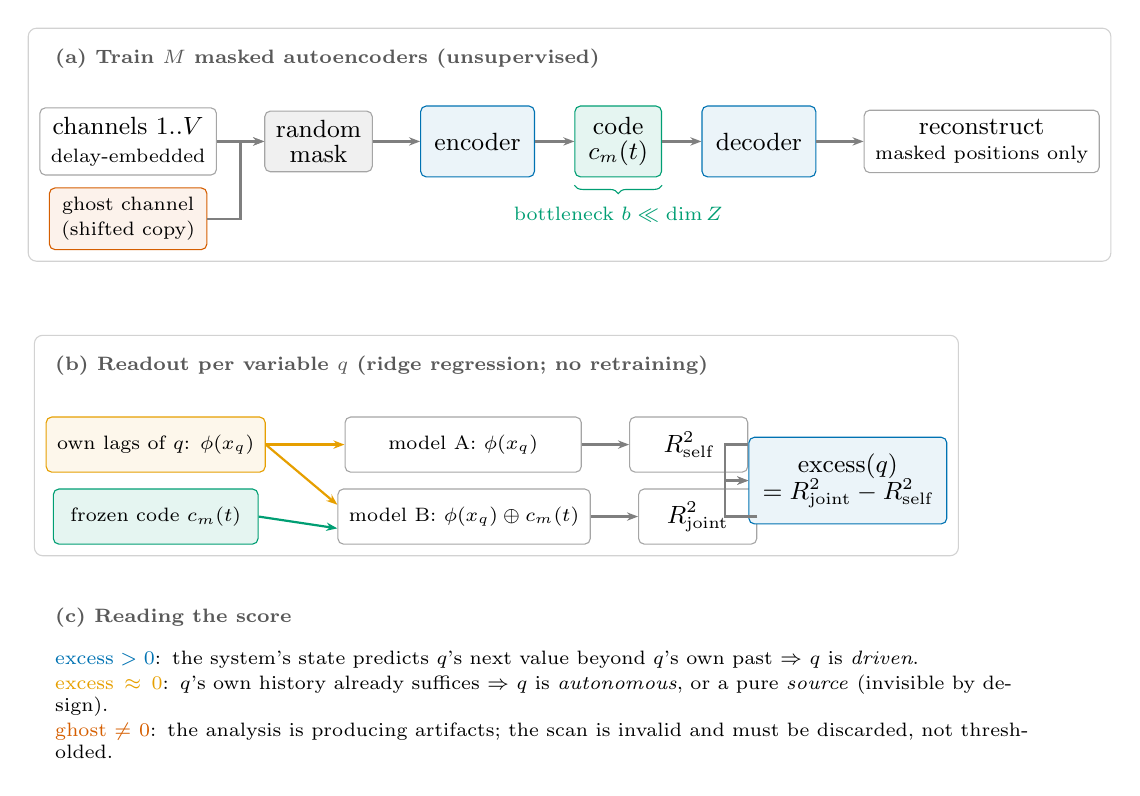
\begin{tikzpicture}[
  font=\small,
  box/.style={draw=cgray!70, rounded corners=2pt, minimum height=7mm,
              inner xsep=4pt, align=center},
  net/.style={draw=cblue, fill=cblue!8, rounded corners=2pt, align=center,
              minimum height=9mm, inner xsep=5pt},
  code/.style={draw=cgreen, fill=cgreen!10, rounded corners=2pt,
               minimum height=9mm, minimum width=11mm, align=center},
  ghost/.style={draw=cverm, fill=cverm!8, rounded corners=2pt, align=center,
                minimum height=7mm, inner xsep=4pt},
  ar/.style={-{Stealth[length=4pt]}, draw=cgray, thick},
  lbl/.style={font=\scriptsize, text=cgray!130},
]

%% ---------- (a) training: masked autoencoder ----------
\node[lbl, anchor=west] (ta) at (0,2.55) {\textbf{(a) Train $M$ masked autoencoders (unsupervised)}};

\node[box, minimum width=20mm] (chan) at (1.05,1.5)
  {channels $1..V$\\[-1pt]\scriptsize delay-embedded};
\node[ghost, minimum width=20mm, below=1.5mm of chan] (gh)
  {\scriptsize ghost channel\\[-2pt]\scriptsize (shifted copy)};

\node[box, fill=cgray!12, minimum width=13mm, right=6mm of chan] (mask)
  {random\\[-2pt]mask};
\node[net, right=6mm of mask] (enc) {encoder};
\node[code, right=5mm of enc] (z) {code\\[-2pt]$c_m(t)$};
\node[net, right=5mm of z] (dec) {decoder};
\node[box, right=6mm of dec, minimum width=17mm] (out)
  {reconstruct\\[-2pt]\scriptsize masked positions only};

\draw[ar] (chan.east) -- (mask.west);
\draw[ar] (gh.east) -| ($(mask.west)+(-3mm,0)$) -- (mask.west);
\draw[ar] (mask) -- (enc);
\draw[ar] (enc) -- (z);
\draw[ar] (z) -- (dec);
\draw[ar] (dec) -- (out);

\draw[decorate, decoration={brace, amplitude=3pt, mirror}, draw=cgreen]
  ($(z.south west)+(0,-1mm)$) -- ($(z.south east)+(0,-1mm)$);
\node[lbl, text=cgreen, below=2.5mm of z.south, align=center]
  {bottleneck $b \ll \dim Z$};

%% ---------- (b) readout: two ridge fits per variable ----------
\node[lbl, anchor=west] (tb) at (0,-1.35)
  {\textbf{(b) Readout per variable $q$ (ridge regression; no retraining)}};

\node[box, minimum width=26mm, fill=corange!8, draw=corange] (own) at (1.4,-2.35)
  {\scriptsize own lags of $q$: $\phi(x_q)$};
\node[code, minimum width=26mm, below=2mm of own, minimum height=7mm] (zz)
  {\scriptsize frozen code $c_m(t)$};

\node[box, minimum width=30mm, right=10mm of own] (m1)
  {\scriptsize model A: $\phi(x_q)$};
\node[box, minimum width=30mm, right=10mm of zz] (m2)
  {\scriptsize model B: $\phi(x_q) \oplus c_m(t)$};

\node[box, right=6mm of m1, minimum width=15mm] (r1) {$R^2_{\text{self}}$};
\node[box, right=6mm of m2, minimum width=15mm] (r2) {$R^2_{\text{joint}}$};

\draw[ar, draw=corange] (own.east) -- (m1.west);
\draw[ar, draw=corange] (own.east) -- ($(m2.west)+(0,1.5mm)$);
\draw[ar, draw=cgreen] (zz.east) -- ($(m2.west)+(0,-1.5mm)$);
\draw[ar] (m1) -- (r1);
\draw[ar] (m2) -- (r2);

\node[draw=cblue, fill=cblue!8, rounded corners=2pt, right=7mm of $(r1)!0.5!(r2)$,
      align=center, minimum height=11mm, inner xsep=5pt] (ex)
  {$\mathrm{excess}(q)$\\[-1pt]$= R^2_{\text{joint}} - R^2_{\text{self}}$};
\draw[ar] (r1.east) -| ($(ex.west)+(-3mm,0)$) -- (ex.west);
\draw[ar] (r2.east) -| ($(ex.west)+(-3mm,0)$) -- (ex.west);

%% ---------- (c) interpretation ----------
\node[lbl, anchor=west] at (0,-4.55) {\textbf{(c) Reading the score}};
\node[align=left, font=\scriptsize, anchor=north west, text width=125mm]
  at (0,-4.85) {
  \textcolor{cblue}{$\mathrm{excess} > 0$}: the system's state predicts $q$'s next
  value beyond $q$'s own past $\Rightarrow$ $q$ is \emph{driven}.\\[1pt]
  \textcolor{corange}{$\mathrm{excess} \approx 0$}: $q$'s own history already
  suffices $\Rightarrow$ $q$ is \emph{autonomous}, or a pure \emph{source}
  (invisible by design).\\[1pt]
  \textcolor{cverm}{ghost $\ne 0$}: the analysis is producing artifacts;
  the scan is invalid and must be discarded, not thresholded.};

\begin{scope}[on background layer]
  \node[fit=(ta)(chan)(gh)(out), draw=cgray!35, rounded corners=3pt,
        inner sep=4pt] {};
  \node[fit=(tb)(own)(zz)(ex), draw=cgray!35, rounded corners=3pt,
        inner sep=4pt] {};
\end{scope}

\end{tikzpicture}
\end{document}
